\begin{figure}[!b]
\centering
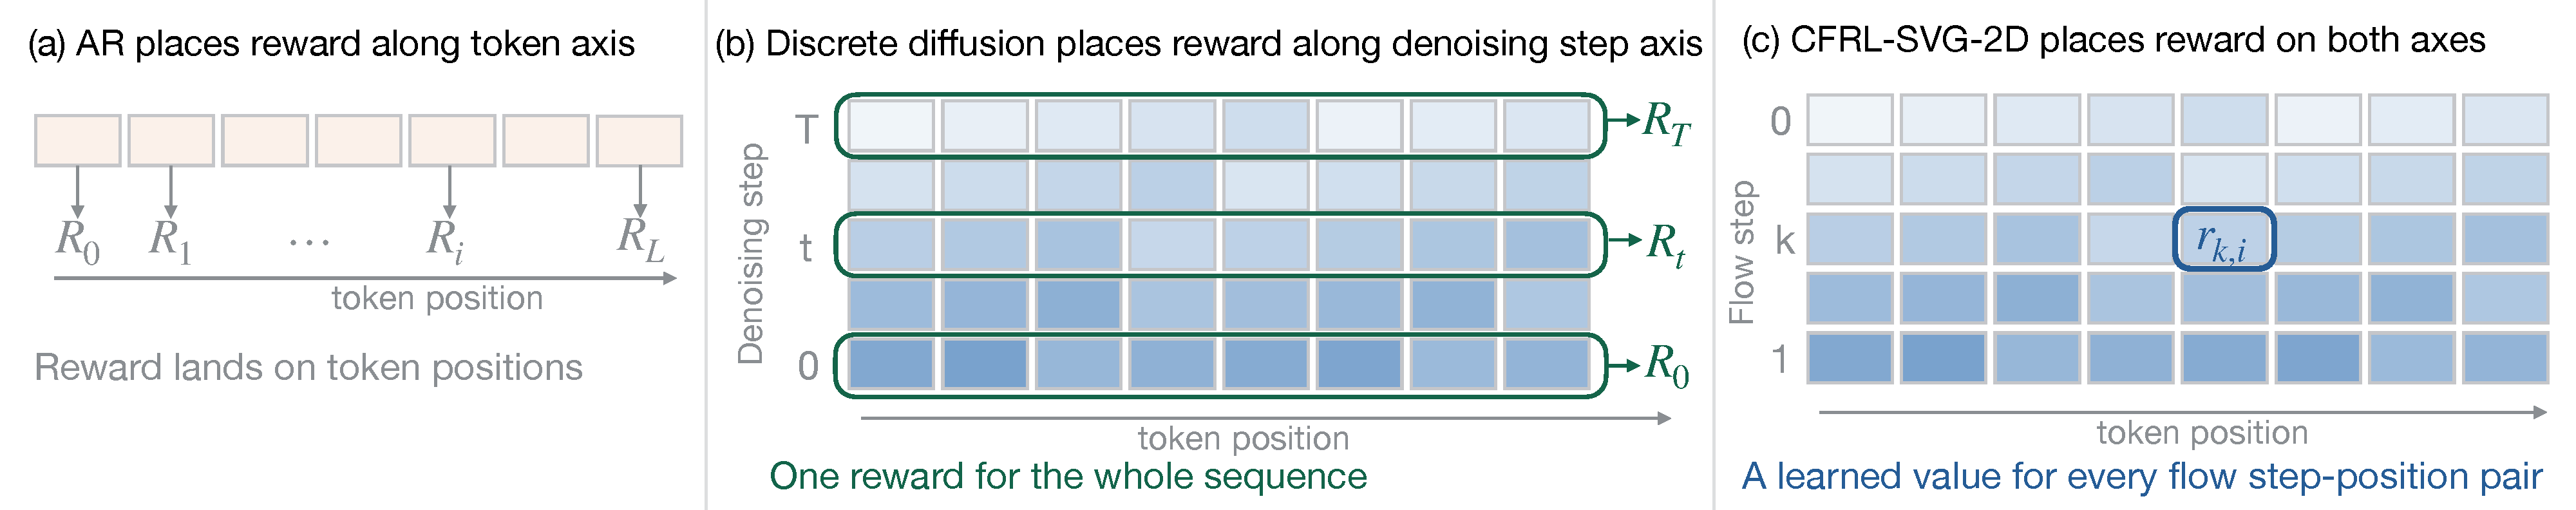
\includegraphics[width=0.84\linewidth]{figures/flow-rl-figure1.pdf}
\caption{Where the reward lands: (a) on the token axis in an AR model; (b) on the step axis in RL for diffusion and flow models; (c) on both in \methodSVGTwoD{}: $R_{k,i}$ for flow step $k$ and position $i$, each an estimate of the whole response's outcome, pooled into $V_\phi$.}
\label{fig:mechanism}
\end{figure}

\subsection{The critic: one value per state, or per state and position}
\label{sec:critic}\label{sec:jpc_scalar}\label{sec:jpc_2d}
The critic takes the state $s_k=(y_k,\hat x_{k-1})$ and the time $\tilde t_k$ as input. Because $\hat x_{k-1}$ is the denoiser's current prediction of the decoded sequence, the critic reuses the denoiser to read it: a copy $\hat X_{\bar\theta}$, initialised from $\theta_{\rm ref}$, fine-tuned once with the head before RL and then held fixed, is evaluated without guidance and gives per-position features $f_i(s_k)=\hat X_{\bar\theta}(y_k,\tilde t_k;\hat x_{k-1})_i\in\mathbb R^d$; a small MLP head $h_\phi$, the part of the critic refit during RL, turns them into a value in one of two orders,
\begin{alignat}{2}
&\text{\methodSVGScalar{}:}&\quad V_\phi(s_k)&=h_\phi\big(\tfrac1{|\mathcal G|}\textstyle\sum_{i\in\mathcal G}f_i(s_k),\,\tilde t_k\big),
\label{eq:critic1d}\\
&\text{\methodSVGTwoD{}:}&\quad V_\phi(s_k)&=\tfrac1{|\mathcal G|}\textstyle\sum_{i\in\mathcal G}R_{k,i},\qquad R_{k,i}=h_\phi\big(f_i(s_k),\tilde t_k\big).
\label{eq:critic2d}
\end{alignat}
A flow model refines all positions at once over $K$ steps, so credit has two axes, \emph{when} along the flow and \emph{where} along the sequence (Figure~\ref{fig:mechanism}). RL for diffusion and flow models treats the whole state as one action indexed by the step \citep{liu2025flowgrpo,xue2025dancegrpo}, as \methodGRPO{} and \methodSVGScalar{} do; \methodSVGTwoD{} indexes the value by both. The actor ascends the pooled value through~(\ref{eq:pw}) in both; the critics differ in the order of head and mean and, through it, in the loss below. The order decides what each position is asked to change. The actor's signal at position $i$ is $\sum_{j}(\partial V_\phi/\partial f_j)(\partial f_j/\partial s_{k,i})$, with $s_{k,i}=(y_{k,i},\hat x_{k-1,i})$ position $i$ of the state, where
\begin{equation}
\text{head after the mean: }\ \frac{\partial V_\phi}{\partial f_j}=\frac{\nabla h_\phi(\bar f)}{|\mathcal G|}\ \ \forall j,\qquad \text{head before the mean: }\ \frac{\partial V_\phi}{\partial f_j}=\frac{\nabla h_\phi(f_j)}{|\mathcal G|},
\label{eq:headgrad}
\end{equation}
with $\bar f$ the mean feature and $\nabla h_\phi$ the gradient in the feature argument. Either every position is pushed along one direction of feature space, the head's slope at the mean, or each along the head's slope at its own reading, the change that would raise its own estimate of success. At a given training step the two updates are similar, because both critics use the same features and outcome labels (Appendices~\ref{app:critic_equiv}, \ref{app:actor_signal}); they diverge over training as the policy evolves and the heads are refitted (Figure~\ref{fig:dyn}). A head on the mean moreover sees the positions only through the bottleneck $\bar f$: it can be written as a mean of per-position readings only if it is affine (Proposition~\ref{prop:additive}).

\paragraph{Supervision without token labels.}
Both critics are trained on states of rollouts labelled with the rollout's outcome $r$, by binary cross-entropy (BCE); the 2D critic minimises
\begin{equation}
\mathcal L_{\rm 2D}(\phi)=\mathbb E_{(s_k,r)}\Big[\tfrac12\,\mathrm{BCE}\big(\mathrm{sig}(V_\phi(s_k)),r\big)+\tfrac12\,\tfrac1{|\mathcal G|}\textstyle\sum_{i\in\mathcal G}\mathrm{BCE}\big(\mathrm{sig}(R_{k,i}),r\big)\Big],
\label{eq:critic2d_loss}
\end{equation}\eqalias{eq:bce}
whereas the scalar critic minimises the first term alone. The first term fits $V_\phi$ to $\mathrm{logit}\,V^\star_k$, the log-odds that the update ascends; the second, present only for the 2D critic, makes every reading a calibrated log-odds on its own, without which the field $R_{k,\cdot}$ would be constrained only through its mean. One reason to expect the field to stay a usable target \emph{under the refit}: a head on the mean is one function of one vector, which the actor can raise by moving that vector wherever the head reads success, whereas a rise of the pooled field has to be carried by $|\mathcal G|$ readings, each taken by the refit head at its own position and, with the second term, each fitted to the outcome. Without the refit either critic is exploited (Table~\ref{tab:critic_design}; Appendices~\ref{app:frozen}, \ref{app:critic_equiv}). $R_{k,i}$ is not a verifier of token $i$: every reading attends over the whole state and predicts the outcome of the whole response, and within a failed response the readings barely tell wrong positions from right ones (Appendix~\ref{app:critic_maps}). What the field changes is the behaviour of the update under joint training (Figure~\ref{fig:dyn}).

\subsection{Architecture and model training}

In the architecture design, the critic $V_\phi$ shares the same transformer with the policy $\phi_\theta$. At step $k$, they both 
take $(\rvz_{t_{k}}, t_k, \rvx_{t_{k-1}}, \rvc)$ as the input and get $L$ token embeddings $\rvh = (h_1, \ldots, h_L)$ after the transformer architecture. 
Then the output of the critic is computed from a mean pooling of these vectors: 
\begin{align}
V_{\phi}(s_k) = \mathrm{sigmoid}(u \cdot \mathrm{mean}(\rvh))
\end{align}
Here $u$ is a learnable parameter included in $\phi$.  



%\subsection{Training the critic with the policy}
During model training, we first pre-train the value function from trajectories sampled with an initial ELF model: the training updates both the 
the transformer and the transformer. In later joint training of both the policy $\pi_\theta$ and the critic $V_\phi$. The samples $(s_k, s_{K+1})$ 
are taken from sampled trajectoires. [TODO: please give a better description how trajectories are sampled]
, then the transformer only receives gradients from $\pi_\theta$, and the critic only trains the projection $u$.  


%NOTE: I don't understand this paragraph, but it seems to contain important information 
%We train the critic jointly with the policy because two things move the condition under which the bias $b_k$ of~(\ref{eq:biasm}) vanishes: 
%as $\theta$ changes, so do the states the policy visits and so does $V^\star_k$ itself, so a critic fitted to an earlier policy is stale even on a state it has seen, and the actor, ascending $V_\phi$ wherever 
%its slope is positive, exploits it. The critic is pre-trained on rollouts of the initial policy, copy and head together, with the first term of~(\ref{eq:critic2d_loss}) for both critics, and 
%Algorithm~\ref{alg:jpc} then refits the head after every actor step, on a replay buffer of the states that fresh rollouts reach at the window's last step $k_{\rm hi}$ alone, 
%where the outcome is most determined by the state; the copy $\bar\theta$ stays fixed (Table~\ref{tab:critic_design}). If the critic's ranking of outcomes on the newest buffer states 
%(its AUC) falls below a floor, the head takes extra steps before the actor moves. The bias paid per step grows with the step size, hence a decaying schedule; and both networks are trained 
%under the sampler to be deployed, since a different sampler is a different chain with different values.

\begin{algorithm}[t]
\caption{\methodSVGScalar{} and \methodSVGTwoD{}: critic~(\ref{eq:critic1d}) or~(\ref{eq:critic2d}); values: Appendix~\ref{app:details}}
\label{alg:jpc}
\small
\begin{algorithmic}[1]
\REQUIRE policy parameters $\theta$; pre-trained critic $V_\phi$ with trainable head parameters $\phi$ on a fixed copy of the denoiser; verifier $r$; sampler $(\gamma,K)$; window $\mathcal W$ with top step $k_{\rm hi}$; buffer $\mathcal B$ and its size $N_{\mathcal B}$; iterations $T$, prompts per iteration $B$, critic minibatch $B'$ and steps $m_{\rm c}$, AUC check every $n_q$ iterations on the newest $N_q$ states with floor $a_0$ and $m'_{\rm c}$ extra steps; learning rates $\eta_\theta,\eta_\phi$
\FOR{iteration $=1,\dots,T$}
  \STATE \textbf{Actor.} For $B$ prompts and one $k\sim\mathcal U(\mathcal W)$: roll out under $(\gamma,K)$ to $s_{k-1}$ without gradients, take the denoiser call at $s_{k-1}$ with gradients to form $s_k$, and set $\theta\leftarrow\theta+\eta_\theta\,\mathrm{AdamW}\big(\nabla_\theta\frac1B\sum_{g=1}^{B}V_\phi(s^g_k)\big)$ \hfill (eq.~\ref{eq:pw}; gradient-norm clipped)
  \STATE \textbf{Buffer.} Roll out $B$ fresh prompts under $(\gamma,K)$ to the end, decode, verify; push each $(s_{k_{\rm hi}},r)$ into $\mathcal B$, keeping the newest $N_{\mathcal B}$
  \STATE \textbf{Critic.} $m_{\rm c}$ head steps $\phi\leftarrow\phi-\eta_\phi\,\mathrm{AdamW}(\nabla_\phi\mathcal L_{\rm 2D})$ on minibatches of $B'$ states of $\mathcal B$; every $n_q$ iterations, $m'_{\rm c}$ more if the AUC of $V_\phi$ on the newest $N_q$ states is below $a_0$ \hfill (eq.~\ref{eq:critic2d_loss}; first term for~(\ref{eq:critic1d}))
\ENDFOR
\end{algorithmic}
\end{algorithm}



\label{sec:loop}
The SVG variants' gains are specific to their training chain and need not transfer to a cheaper chain through the same denoiser (Appendix~\ref{app:samplers}). An optional amortisation step transfers them to other samplers through the supervised objective, which trains the denoiser at every time $t$: a round samples the policy on a pool of unlabelled prompts, keeps the verified, distinct responses, and fine-tunes the model on them with ELF's loss (Algorithm~\ref{alg:loop}, Appendix~\ref{app:loop}). This is rejection-sampling fine-tuning \citep{yuan2023rft}, the M-step of an EM view of the per-prompt reward in~(\ref{eq:objective}), whose bound is tight at the current model for plain sampling before de-duplication (Proposition~\ref{prop:em}). A round learns only from prompts with accepted responses, so its reach is limited by the pool's coverage, which the 2D critic can help expand: it uses its most pessimistic position, $\min_{i}\mathrm{sig}(R_{k,i})$, to prune parallel chains and to guide the state before decoding, so that pools can be drawn with a cheap chain (Appendix~\ref{app:loop}).
